\chapter{Lược đồ E--R và mô tả dữ liệu}

\section{Lược đồ E--R}
Mô hình trong báo cáo gồm 20 bảng nghiệp vụ thuộc phương án rút gọn. Để sơ đồ dễ đọc, lược đồ E--R được trình bày qua ba góc nhìn có dùng chung một số bảng: nghiệp vụ lõi, bán hàng POS, và phân công/kiểm toán/thông báo. Tập hợp ba góc nhìn bao phủ đủ 20 bảng; mỗi đường nối biểu diễn một quan hệ khóa ngoại.

\begin{landscape}
\begin{figure}[p]
  \centering
  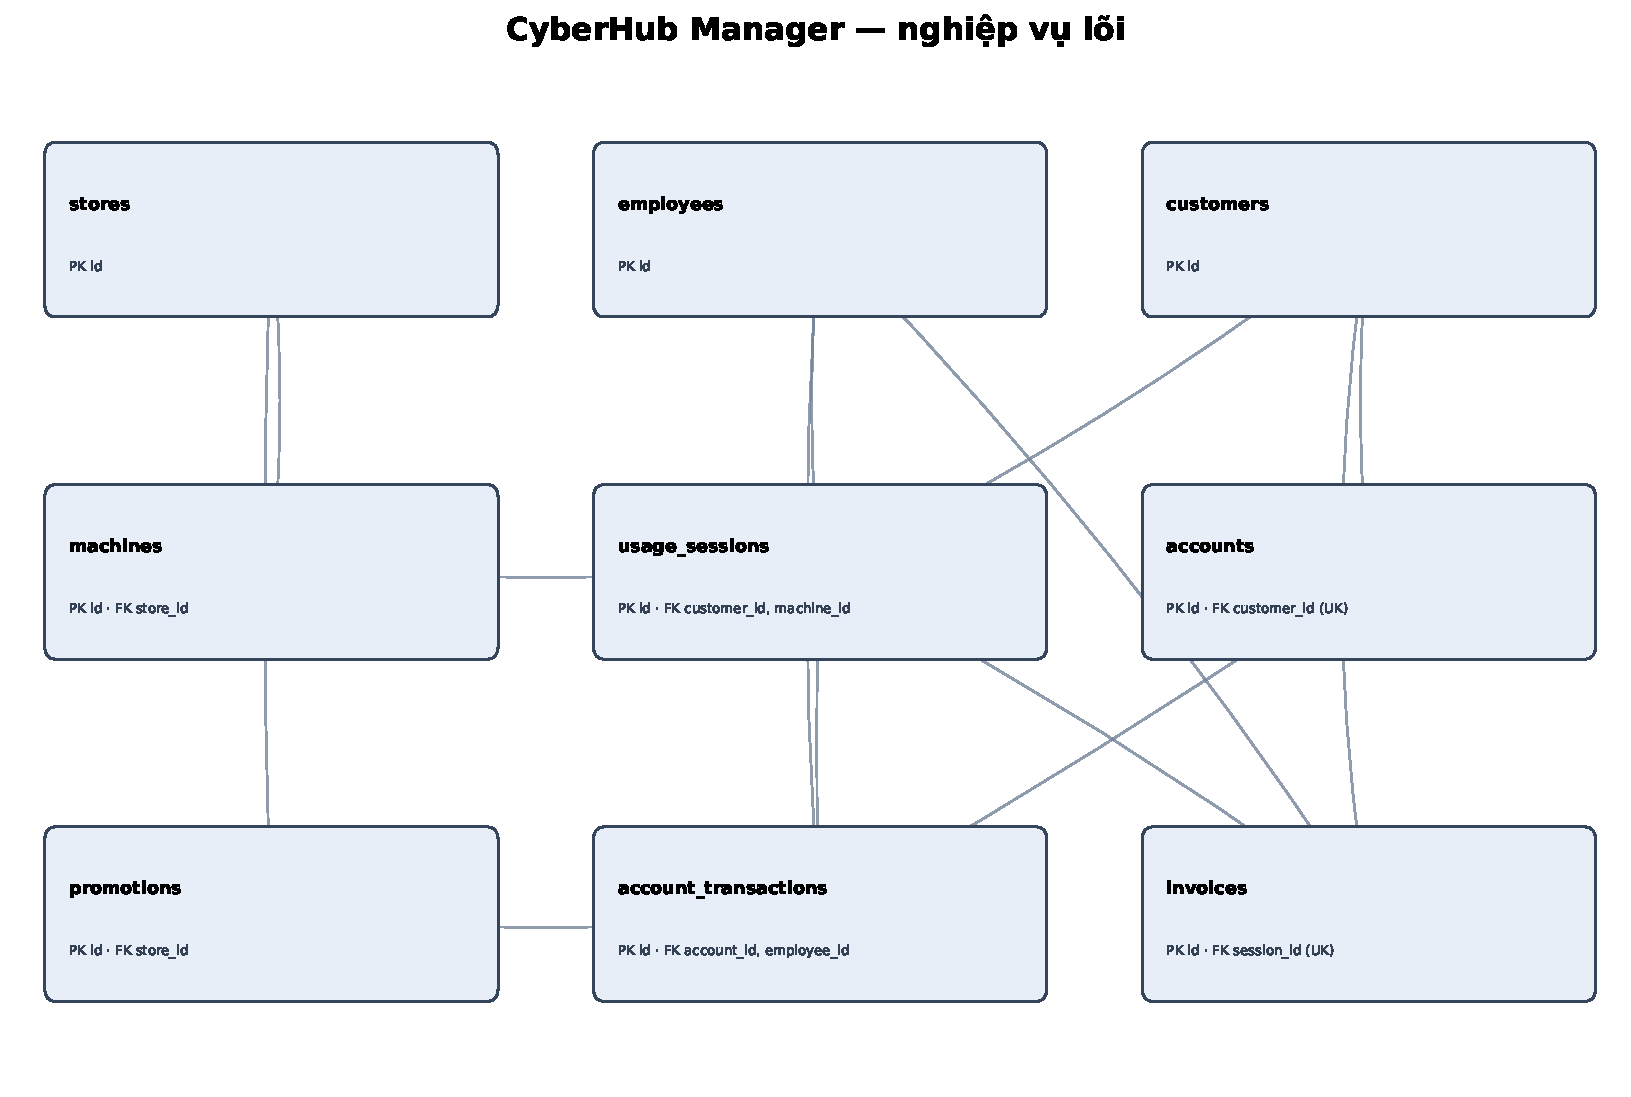
\includegraphics[width=0.95\linewidth,height=0.78\textheight,keepaspectratio]{figures/erd_20_core.pdf}
  \caption{Lược đồ E--R cho nghiệp vụ lõi: khách hàng, tài khoản và phiên máy}
  \label{fig:erd-20-core}
\end{figure}
\end{landscape}
\clearpage
\begin{landscape}
\begin{figure}[p]
  \centering
  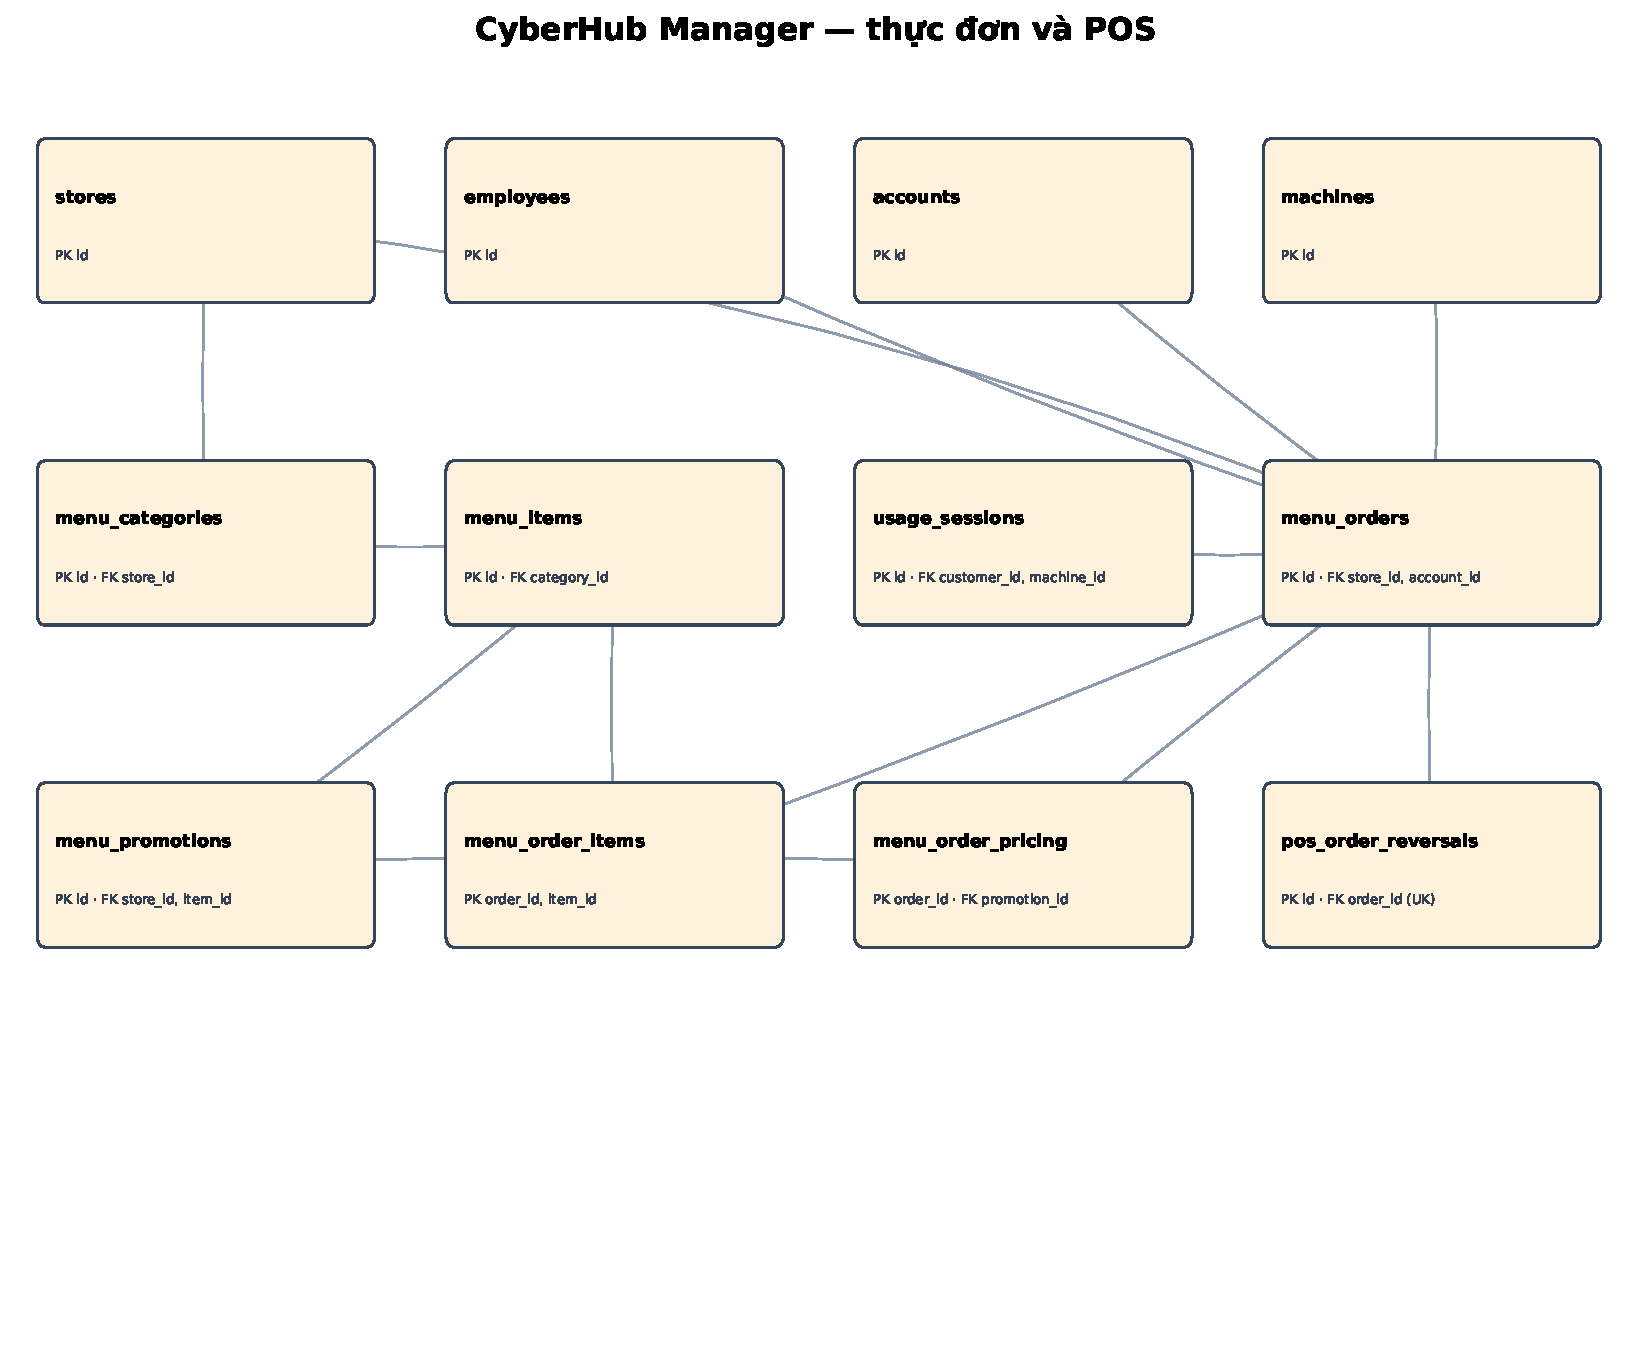
\includegraphics[width=0.95\linewidth,height=0.78\textheight,keepaspectratio]{figures/erd_20_pos.pdf}
  \caption{Lược đồ E--R cho thực đơn và bán hàng POS}
  \label{fig:erd-20-pos}
\end{figure}
\end{landscape}
\clearpage
\begin{landscape}
\begin{figure}[p]
  \centering
  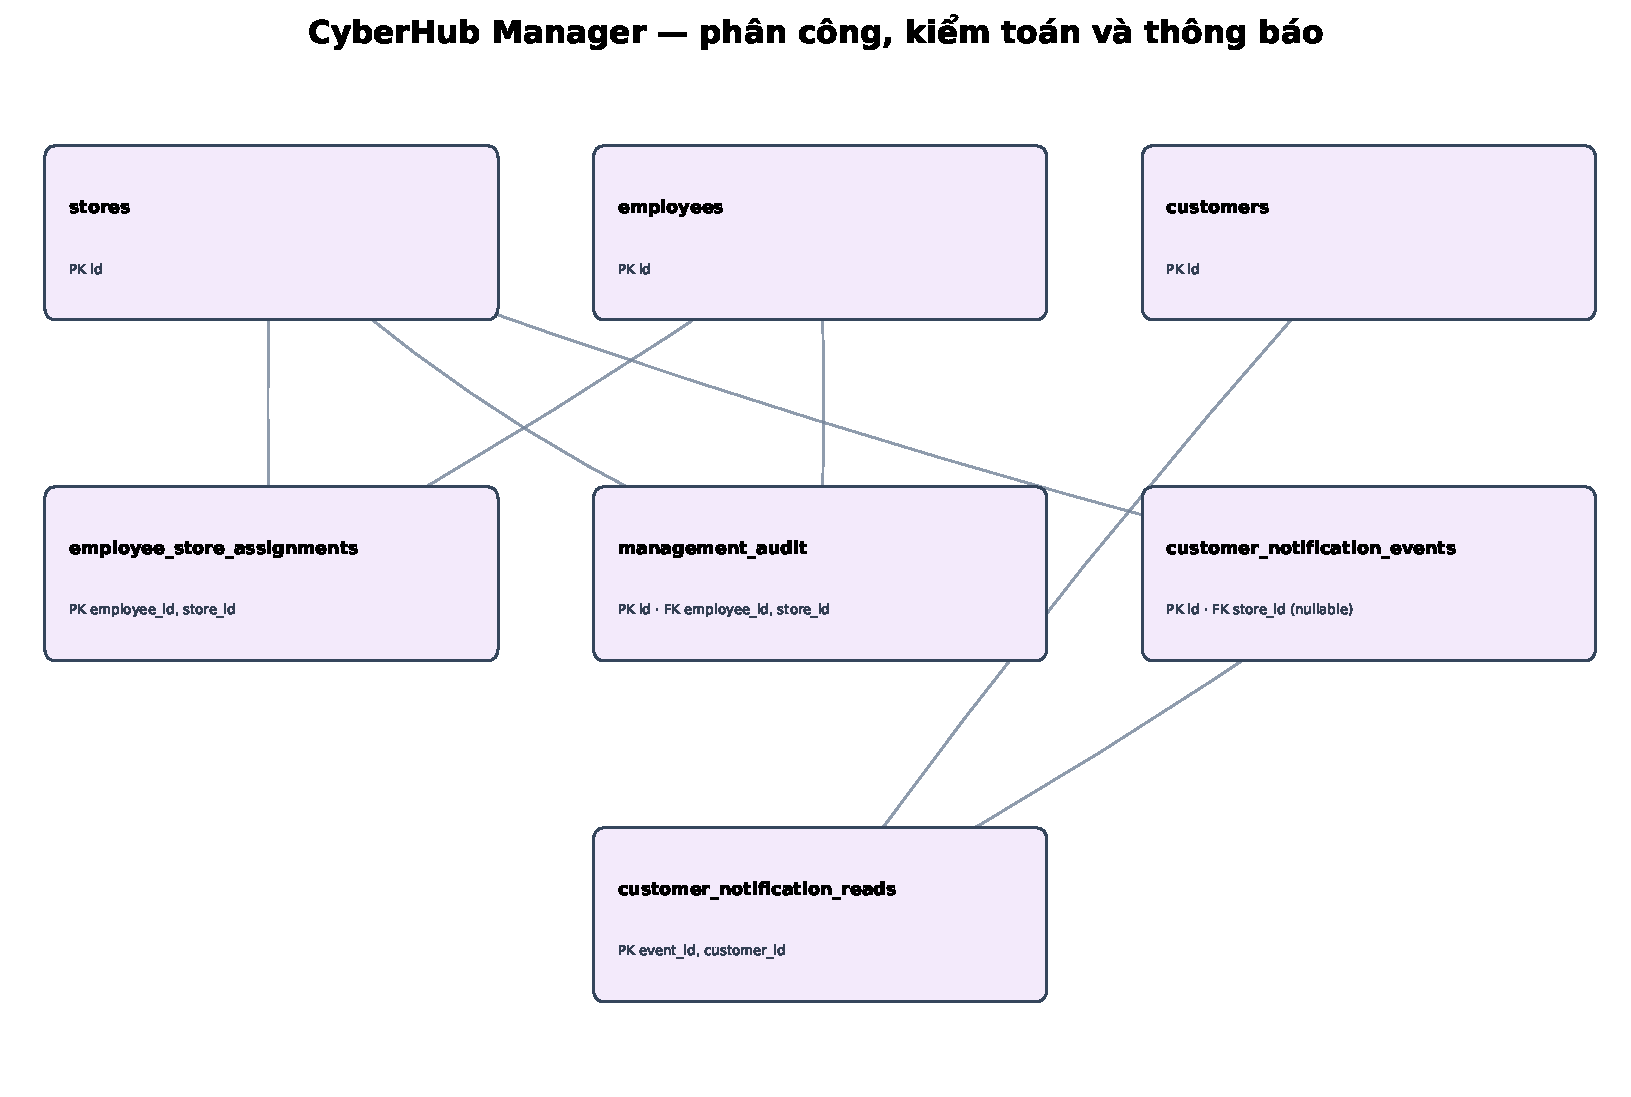
\includegraphics[width=0.95\linewidth,height=0.78\textheight,keepaspectratio]{figures/erd_20_support.pdf}
  \caption{Lược đồ E--R cho phân công nhân viên, kiểm toán và thông báo}
  \label{fig:erd-20-support}
\end{figure}
\end{landscape}
\clearpage

\section{Các thông tin thực thể}
Các thuộc tính dưới đây là những thuộc tính cốt lõi được chọn cho mô hình quan hệ trong báo cáo. PK là khóa chính, FK là khóa ngoại và UK là ràng buộc duy nhất. Những điều kiện được ghi là đề xuất cần được hiện thực trong DDL tương ứng.

\subsection{Cửa hàng và nhân viên}
\begin{description}[leftmargin=3.7cm,labelwidth=3.5cm,style=nextline]
  \item[\texttt{stores}] Lưu thông tin cửa hàng. \textbf{Thuộc tính:} \texttt{id}, \texttt{code}, \texttt{name}, \texttt{address}, \texttt{status}. \textbf{Quan hệ:} một cửa hàng có nhiều máy, nhóm món, món, đơn hàng, giao dịch và hóa đơn; liên kết nhiều--nhiều với nhân viên qua \texttt{employee\_store\_assignments}. \textbf{Ràng buộc:} \texttt{id} là PK; \texttt{code} là UK.
  \item[\texttt{employees}] Lưu thông tin đăng nhập và hồ sơ cơ bản của nhân viên. \textbf{Thuộc tính:} \texttt{id}, \texttt{username}, \texttt{full\_name}, \texttt{phone}, \texttt{role}, \texttt{status}. \textbf{Quan hệ:} liên kết với cửa hàng qua \texttt{employee\_store\_assignments}; có thể được ghi nhận là nhân viên mở/đóng phiên, xử lý giao dịch, lập hóa đơn, thực hiện thao tác quản trị hoặc xử lý yêu cầu hoàn/hủy đơn. \textbf{Ràng buộc:} \texttt{id} là PK; \texttt{username} là UK.
  \item[\texttt{employee\_store\_assignments}] Lưu việc phân công nhân viên cho cửa hàng. \textbf{Thuộc tính:} \texttt{employee\_id}, \texttt{store\_id}, \texttt{granted\_by}, \texttt{granted\_at}. \textbf{Quan hệ:} mỗi bản ghi tham chiếu một nhân viên và một cửa hàng; \texttt{granted\_by} tham chiếu nhân viên cấp quyền. \textbf{Ràng buộc:} PK ghép \texttt{(employee\_id, store\_id)}; các mã tham chiếu là FK.
  \item[\texttt{management\_audit}] Ghi nhận thao tác quản trị. \textbf{Thuộc tính:} \texttt{id}, \texttt{employee\_id}, \texttt{store\_id}, \texttt{action}, \texttt{entity\_type}, \texttt{entity\_id}, \texttt{created\_at}. \textbf{Quan hệ:} mỗi bản ghi liên kết với nhân viên và cửa hàng thực hiện thao tác. \textbf{Ràng buộc:} \texttt{id} là PK; \texttt{employee\_id} và \texttt{store\_id} là FK.
\end{description}

\subsection{Khách hàng, tài khoản và phiên sử dụng máy}
\begin{description}[leftmargin=3.7cm,labelwidth=3.5cm,style=nextline]
  \item[\texttt{customers}] Lưu hồ sơ khách hàng. \textbf{Thuộc tính:} \texttt{id}, \texttt{code}, \texttt{full\_name}, \texttt{phone}, \texttt{email}, \texttt{status}. \textbf{Quan hệ:} một khách hàng có tối đa một tài khoản; khách hàng có thể có nhiều phiên sử dụng và liên kết với thông báo đã đọc. \textbf{Ràng buộc:} \texttt{id} là PK; \texttt{code} và \texttt{phone} là UK.
  \item[\texttt{accounts}] Lưu tài khoản và số dư của khách hàng. \textbf{Thuộc tính:} \texttt{id}, \texttt{customer\_id}, \texttt{code}, \texttt{username}, \texttt{balance}, \texttt{status}. \textbf{Quan hệ:} mỗi tài khoản thuộc về một khách hàng; tài khoản được tham chiếu bởi giao dịch và đơn hàng. \textbf{Ràng buộc:} \texttt{id} là PK; \texttt{customer\_id} là FK và UK; \texttt{code} và \texttt{username} là UK.
  \item[\texttt{machines}] Lưu máy tính thuộc cửa hàng. \textbf{Thuộc tính:} \texttt{id}, \texttt{store\_id}, \texttt{code}, \texttt{room\_type}, \texttt{status}, \texttt{hourly\_rate}. \textbf{Quan hệ:} mỗi máy thuộc một cửa hàng và có thể được tham chiếu bởi nhiều phiên; đơn hàng có thể liên kết máy nếu có. \textbf{Ràng buộc:} \texttt{id} là PK; \texttt{store\_id} là FK; cặp \texttt{(store\_id, code)} là UK; \texttt{hourly\_rate} không âm.
  \item[\texttt{usage\_sessions}] Ghi nhận phiên sử dụng máy. \textbf{Thuộc tính:} \texttt{id}, \texttt{customer\_id}, \texttt{machine\_id}, \texttt{opened\_by}, \texttt{closed\_by}, \texttt{started\_at}, \texttt{ended\_at}, \texttt{cost}, \texttt{status}. \textbf{Quan hệ:} mỗi phiên gắn với khách hàng và máy; nhân viên mở/đóng phiên được tham chiếu nếu có; phiên có thể liên quan đến giao dịch, hóa đơn và đơn món. \textbf{Ràng buộc:} \texttt{id} là PK; các mã khách hàng, máy và nhân viên là FK; thời điểm kết thúc không sớm hơn thời điểm bắt đầu. Một máy hoặc khách hàng không nên có hai phiên đang hoạt động cùng lúc.
  \item[\texttt{account\_transactions}] Ghi các giao dịch trên tài khoản. \textbf{Thuộc tính:} \texttt{id}, \texttt{account\_id}, \texttt{employee\_id}, \texttt{session\_id}, \texttt{store\_id}, \texttt{promotion\_id}, \texttt{type}, \texttt{amount}, \texttt{created\_at}. \textbf{Quan hệ:} giao dịch liên kết với tài khoản, nhân viên và cửa hàng; phiên và khuyến mãi có thể không có giá trị. \textbf{Ràng buộc:} \texttt{id} là PK; các mã tham chiếu là FK. Quy ước dấu của \texttt{amount} cần thống nhất với \texttt{type}.
  \item[\texttt{invoices}] Lưu hóa đơn cho phiên sử dụng. \textbf{Thuộc tính:} \texttt{id}, \texttt{session\_id}, \texttt{customer\_id}, \texttt{employee\_id}, \texttt{store\_id}, \texttt{usage\_cost}, \texttt{total\_amount}, \texttt{status}, \texttt{issued\_at}. \textbf{Quan hệ:} hóa đơn liên kết với phiên, khách hàng, nhân viên lập và cửa hàng. \textbf{Ràng buộc:} \texttt{id} là PK; các mã tham chiếu là FK; \texttt{session\_id} là UK nên mỗi phiên có tối đa một hóa đơn.
  \item[\texttt{promotions}] Lưu chương trình khuyến mãi liên quan đến giao dịch tài khoản. \textbf{Thuộc tính:} \texttt{id}, \texttt{store\_id}, \texttt{code}, \texttt{minimum\_amount}, \texttt{bonus\_percent}, \texttt{starts\_at}, \texttt{ends\_at}, \texttt{status}. \textbf{Quan hệ:} chương trình thuộc cửa hàng và có thể được giao dịch tham chiếu. \textbf{Ràng buộc:} \texttt{id} là PK; \texttt{store\_id} là FK; cặp \texttt{(store\_id, code)} là UK; thời điểm kết thúc không sớm hơn thời điểm bắt đầu.
\end{description}

\subsection{Thực đơn và bán hàng tại quầy}
\begin{description}[leftmargin=3.7cm,labelwidth=3.5cm,style=nextline]
  \item[\texttt{menu\_categories}] Lưu nhóm món của cửa hàng. \textbf{Thuộc tính:} \texttt{id}, \texttt{store\_id}, \texttt{name}, \texttt{page}, \texttt{status}. \textbf{Quan hệ:} mỗi nhóm thuộc một cửa hàng và có thể được nhiều món tham chiếu. \textbf{Ràng buộc:} \texttt{id} là PK; \texttt{store\_id} là FK; cặp \texttt{(store\_id, name)} là UK.
  \item[\texttt{menu\_items}] Lưu các món được bán. \textbf{Thuộc tính:} \texttt{id}, \texttt{store\_id}, \texttt{category\_id}, \texttt{name}, \texttt{price}, \texttt{status}. \textbf{Quan hệ:} món thuộc cửa hàng và nhóm món; được tham chiếu trong dòng đơn và chương trình khuyến mãi món. \textbf{Ràng buộc:} \texttt{id} là PK; \texttt{store\_id} và \texttt{category\_id} là FK; giá không âm.
  \item[\texttt{menu\_orders}] Lưu đơn món. \textbf{Thuộc tính:} \texttt{id}, \texttt{store\_id}, \texttt{account\_id}, \texttt{session\_id}, \texttt{machine\_id}, \texttt{handled\_by}, \texttt{status}, \texttt{total\_amount}, \texttt{created\_at}. \textbf{Quan hệ:} đơn thuộc cửa hàng, có tài khoản thanh toán và nhân viên xử lý; phiên và máy liên quan có thể không có giá trị; các món trong đơn được lưu ở \texttt{menu\_order\_items}. \textbf{Ràng buộc:} \texttt{id} là PK; các mã tham chiếu là FK.
  \item[\texttt{menu\_order\_items}] Lưu từng dòng món của đơn. \textbf{Thuộc tính:} \texttt{order\_id}, \texttt{item\_id}, \texttt{item\_name}, \texttt{unit\_price}, \texttt{quantity}. \textbf{Quan hệ:} mỗi dòng thuộc một đơn hàng và tham chiếu một món; bảng này biểu diễn quan hệ nhiều--nhiều giữa đơn hàng và món. \textbf{Ràng buộc:} PK ghép \texttt{(order\_id, item\_id)}; hai mã là FK; \texttt{quantity} lớn hơn 0; đơn giá không âm. Tên món và đơn giá được lưu tại thời điểm đặt.
  \item[\texttt{menu\_promotions}] Lưu khuyến mãi áp dụng cho món tại cửa hàng. \textbf{Thuộc tính:} \texttt{id}, \texttt{store\_id}, \texttt{item\_id}, \texttt{code}, \texttt{kind}, \texttt{value}, \texttt{starts\_at}, \texttt{ends\_at}. \textbf{Quan hệ:} khuyến mãi thuộc cửa hàng, áp dụng cho món và có thể được tham chiếu từ dữ liệu tính giá đơn. \textbf{Ràng buộc:} \texttt{id} là PK; \texttt{store\_id} và \texttt{item\_id} là FK; thời điểm kết thúc không sớm hơn thời điểm bắt đầu.
  \item[\texttt{menu\_order\_pricing}] Lưu kết quả tính giá và khuyến mãi của đơn. \textbf{Thuộc tính:} \texttt{order\_id}, \texttt{promotion\_id}, \texttt{discount\_amount}, \texttt{final\_amount}. \textbf{Quan hệ:} mỗi bản ghi thuộc một đơn và có thể tham chiếu khuyến mãi món. \textbf{Ràng buộc:} \texttt{order\_id} là PK và FK; \texttt{promotion\_id} là FK, có thể để trống; số tiền cuối cùng không âm.
  \item[\texttt{pos\_order\_reversals}] Lưu yêu cầu hoàn/hủy đơn POS. \textbf{Thuộc tính:} \texttt{id}, \texttt{order\_id}, \texttt{store\_id}, \texttt{requested\_by}, \texttt{decided\_by}, \texttt{status}, \texttt{reason}, \texttt{created\_at}. \textbf{Quan hệ:} mỗi yêu cầu gắn với đơn, cửa hàng và nhân viên yêu cầu/quyết định. \textbf{Ràng buộc:} \texttt{id} là PK; các mã tham chiếu là FK; \texttt{order\_id} là UK nên mỗi đơn có tối đa một hồ sơ hoàn/hủy.
\end{description}

\subsection{Thông báo khách hàng}
\begin{description}[leftmargin=3.7cm,labelwidth=3.5cm,style=nextline]
  \item[\texttt{customer\_notification\_events}] Lưu nội dung thông báo được tạo. \textbf{Thuộc tính:} \texttt{id}, \texttt{store\_id}, \texttt{title}, \texttt{message}, \texttt{event\_type}, \texttt{created\_at}. \textbf{Quan hệ:} thông báo có thể gắn với một cửa hàng hoặc áp dụng toàn hệ thống; liên kết với khách hàng qua \texttt{customer\_notification\_reads}. \textbf{Ràng buộc:} \texttt{id} là PK; \texttt{store\_id} là FK và có thể để trống.
  \item[\texttt{customer\_notification\_reads}] Lưu khách hàng đã đọc thông báo và thời điểm đọc. \textbf{Thuộc tính:} \texttt{event\_id}, \texttt{customer\_id}, \texttt{read\_at}. \textbf{Quan hệ:} mỗi bản ghi liên kết một thông báo với một khách hàng. \textbf{Ràng buộc:} PK ghép \texttt{(event\_id, customer\_id)}; cả hai thuộc tính là FK.
\end{description}

\section{Kết luận chương}
Lược đồ E--R và phần mô tả trên trình bày 20 bảng nghiệp vụ trong phạm vi báo cáo, bao gồm khóa, thuộc tính cốt lõi, quan hệ chính và một số ràng buộc dữ liệu. Các quan hệ nhiều--nhiều được biểu diễn qua bảng liên kết hoặc bảng chi tiết phù hợp. Mô hình tập trung vào vận hành cửa hàng Internet, sử dụng máy và bán món tại quầy.
